\chapter{Domain Driven Design}
Domain Driven Design ist ein Ansatz der Software Entwicklung, bei dem die Domäne und deren Logik im Mittelpunkt steht. Dabei hilft DDD der Komplexität von Software vorzubeugen, indem es den Fokus auf das Verständnis der Domäne legt. \cite{ddd.2003}
\section{Ubiquitous Language}
% 4 Beispiele für die Ubiquitous Language; jeweils Bezeichnung, Bedeutung und kurze Begründung, warum es zur Ubiquitous Language gehört
Ubiquitous Language ist ein zentrales Konzept im Domain-Driven Design und bezieht sich auf eine gemeinsame, konsistente Sprache, die von allen Beteiligten im Projekt verwendet wird, um die Domäne und ihre Anforderungen zu beschreiben. Diese einheitliche Sprache soll Kommunikationsprobleme zwischen Entwicklern, Fachexperten, Stakeholdern und anderen Teammitgliedern vermeiden und ein gemeinsames Verständnis der Domäne fördern. In der Praxis bedeutet dies, dass die Begriffe, die in der Geschäftsdomäne verwendet werden, konsistent in den Diskussionen, Dokumentationen und im Code selbst verwendet werden sollten. Ubiquitous Language wird im gesamten Entwicklungsprozess eingesetzt, von der Anforderungsanalyse über das Design bis hin zur Implementierung.
Im Folgenden wird die Ubiquitous Language des Simpsons Quiz Projekts vorgestellt.
\begin{itemize}
    \item Charakter: Ein Charakter ist eine Person der Simpsons Serie. Dabei ist es egal ob es sich um einen Hauptcharakter oder einen Nebencharakter handelt.
    \item Picture: Ein Picture ist ein Bild, welches einem Charakter der Serie zugeordnet ist.
    \item Workplace: Ein Workplace ist ein Arbeitsplatz, welcher einem Charakter der Serie zugeordnet ist.
    \item Home: Ein Home ist ein Wohnort, welcher einem Charakter der Serie zugeordnet ist.
    \item LuxuryFood: Ein LuxuryFood ist das Lieblingsessen, welches einem Charakter der Serie zugeordnet ist.
    \item Transport: Ein Transport ist das präferierte  Transportmittel, welches einem Charakter der Serie zugeordnet ist.
\end{itemize}
Die Begriffe zählen zur Ubiquitous Language, da sie essentiell für das Verständnis des Simpsons Quiz sind und die Hauptmerkmale des Aufbaus der jeweiligen Figur im Rahmen des Quiz darstellen. Dabei werden sie bei der Implementierung als Gruppierung der einzelnen Attribute verwendet.
\section{Entities}
% UML, Beschreibung und Begründung des Einsatzes einer Entity; falls keine Entity vorhanden: ausführliche Begründung, warum es keines geben kann/hier nicht sinnvoll ist
Entitäten repräsentieren Objekte, die innerhalb einer Geschäftsdomäne eine eindeutige Identität besitzen. Im Gegensatz zu Value Objects, die nur durch ihre Attribute definiert sind, haben Entitäten eine Identität, die unabhängig von ihren Eigenschaften ist. Das bedeutet, dass selbst wenn sich der Zustand einer Entität im Laufe der Zeit ändert, ihre Identität konstant bleibt. Beispiele für Entitäten können Kunden, Produkte, Bestellungen oder Mitarbeiter sein. In all diesen Fällen ist die Identität des Objekts entscheidend, um es von anderen Objekten desselben Typs unterscheiden zu können. Im Simpsons Quiz stellen Charakter, Workplace, Home, LuxuryFood und Transport Entitäten dar.
\newpage

\section{Value Objects}
% UML, Beschreibung und Begründung des Einsatzes eines Value Objects; falls kein Value Object vorhanden: ausführliche Begründung, warum es keines geben kann/hier nicht sinnvoll ist
Value Objects sind ein wichtiger Bestandteil von Domain-Driven Design (DDD) und repräsentieren Objekte, die keine eigene Identität haben und ausschließlich durch ihre Eigenschaften oder Attribute definiert sind. Im Gegensatz zu Entitäten, die eine eindeutige Identität besitzen und deren Zustand sich im Laufe der Zeit ändern kann, sind Value
Objects unveränderlich und können bei Bedarf einfach ersetzt werden. Im Simpsons Quiz stellen die einzelne Charaktere des Spiels Value Objects dar. Sie sind anhand ihrer Attribute wie Arbeitsplätze, Vorlieben oder Zitaten einzigartig und können nur durch einen anderen Charakter ersetzt, aber nicht verändert werden.
\begin{figure}[ht]
    \centering
    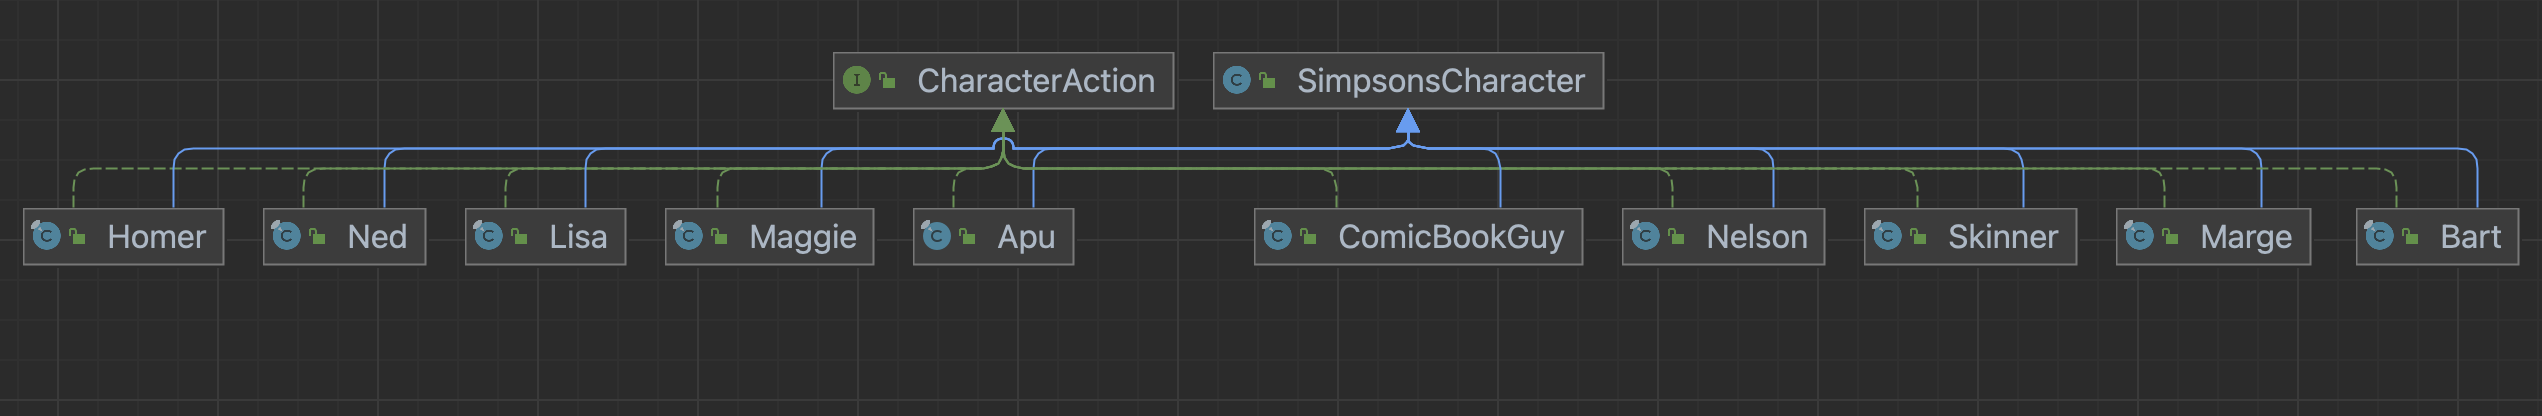
\includegraphics[width=0.9\textwidth]{Bilder/charakter.png}
    \caption{UML Diagramm für Value Objects}
    \label{fig:ValueObject}
\end{figure}

\section{Repositories}

Repositories vermitteln zwischen der Domäne und dem Modell und stellen Methoden bereit um Aggregates aus dem Persistenzspeicher zu lesen oder zu speichern. Im Simpsons Quiz werden keine Repositories verwendet, da die Abfrage des Aggregates bereits alle Informationen liefert und somit eine weitere Abstraktionsebene überflüssig macht. 
\newpage
\section{Aggregates}
% UML, Beschreibung und Begründung des Einsatzes eines Aggregates; falls kein Aggregate vorhanden: ausführliche Begründung, warum es keines geben kann/hier nicht sinnvoll ist
Aggregates beziehen sich auf eine Gruppe von zusammenhängenden Entitäten und Value Objects, die eine konsistente Geschäftseinheit bilden. Dabei ist genau geregelt, welche Entitäten und Value Objects zu einem Aggregate gehören und welche nicht, um die Abhängigkeiten abzubilden. \newline
Im Simpsons Quiz gibt es das Aggregate UserBuild, welches aus den Entitäten Charakter, Workplace, Home, LuxuryFood und Transport besteht und mit den Value Objects die Spiel Figur zusammenstellt.
